\documentclass[aspectratio=169]{beamer}

\usetheme{DUNE}
\beamertemplatenavigationsymbolsempty
\setbeamertemplate{frametitle}{\insertframetitle}

\usepackage[T1]{fontenc}
\usepackage[utf8]{inputenc}
\usepackage{graphicx,booktabs,array,hyperref}
\usepackage{siunitx}
\usepackage{appendixnumberbeamer}
\usepackage[dvipsnames]{xcolor}

\title[March 2026 Cold Box]{March 2026 Cold Box\\Data-taking status summary}
\subtitle{Noise runs, 270 nm SPE-oriented scans, and 367 nm dynamic-range scans}
\author{Manuel Arroyave, Terri Shaw, Dante Totani, Mariya Mollova}
\date{March 20, 2026}

\begin{document}

\begin{frame}
  \titlepage
\end{frame}

\begin{frame}{Requested scope vs. data categories taken}
\footnotesize
\textbf{Requested in the March 6 plan}
\begin{itemize}
  \item Noise characterization with LED off: FFT, baseline STD, baseline offset.
  \item Low-light LED scans to set a working point around 1 average PE.
  \item VGAIN and bias scans to extract SPE response and SNR.
  \item High-light LED scans to probe dynamic range and saturation.
\end{itemize}

\vspace{1mm}
\textbf{What we actually accumulated}
\begin{itemize}
  \item \textbf{Noise runs:} dark VGAIN scans plus oscilloscope captures under several electrical configurations.
  \item \textbf{270 nm scans:} low-light tuning scans and targeted VGAIN/bias matrices for SPE-oriented studies.
  \item \textbf{367 nm scans:} high-light scans used to push channels toward dynamic-range and saturation studies.
  \item \textbf{Coverage picture:} working assumption is that VD channels 0--7 and HD channels 8--15 are largely covered; the systematic campaign still missing is mainly SoF / AFE2, channels 16--23.
\end{itemize}
\end{frame}

\begin{frame}{Nature of the noise runs}
\footnotesize
\begin{itemize}
  \item These are \textbf{LED-off} runs meant to separate readout/electronics noise from LED and signal-shape effects.
  \item The main observables are \textbf{baseline STD} and \textbf{FFT floor / spectral structure} as a function of VGAIN.
  \item The run family includes standard dark scans, detector-connected variants, and cable/choke follow-ups.
  \item This is the dataset used to compare noise between measurements and to flag obvious outliers before interpreting SPE scans.
\end{itemize}
\end{frame}
\begin{frame}
  \vspace{1mm}
  \centering
  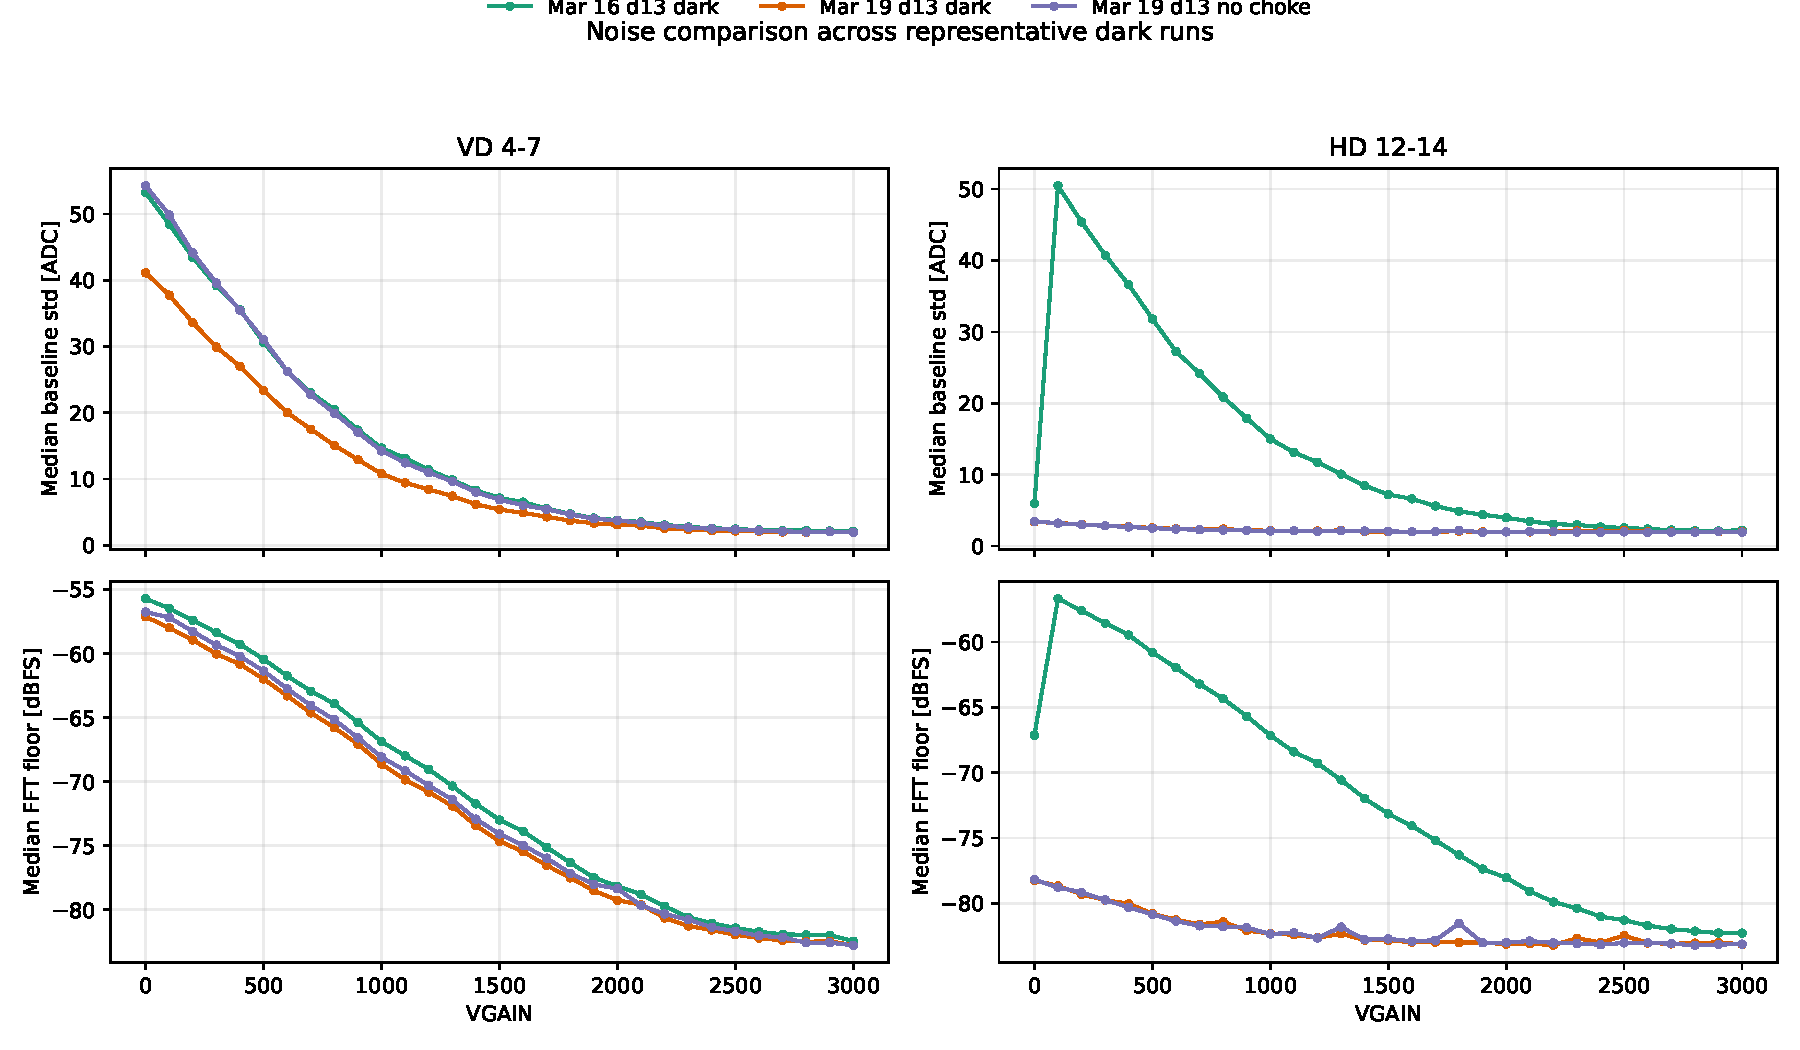
\includegraphics[width=0.94\linewidth]{figures/noise_comparison_summary.pdf}
\end{frame}

\begin{frame}{270 nm scans: purpose and workflow}
\footnotesize
\begin{itemize}
  \item The 270 nm scans were used as the \textbf{SPE-oriented working dataset}.
  \item First step: scan LED intensity channel-by-channel to find a usable low-light operating point with visible pedestal / first-PE structure.
  \item Second step: with those fixed intensities, run \textbf{VGAIN scans} and \textbf{VGAIN-bias matrices} to map SPE response, SNR trends, and the dependence on front-end settings.
  \item In practice, this produced:
  \begin{itemize}
    \item VD tuning scans for channels 0--7.
    \item HD tuning scans and dedicated matrices for channels 12--15.
    \item Partial / resumed 2D matrices for VD follow-up studies.
  \end{itemize}
\end{itemize}

\vspace{1mm}
\scriptsize
\begin{tabular}{>{\raggedright\arraybackslash}p{0.33\linewidth} >{\raggedright\arraybackslash}p{0.61\linewidth}}
\toprule
\textbf{Representative data} & \textbf{Purpose} \\
\midrule
\texttt{20260317\_daphne-13\_led\_vgain\_bias\_scan} & HD matrix, 270 nm, fixed LED per channel group, VGAIN and AFE1 bias scan for SPE-oriented evaluation \\
\texttt{20260319\_vd\_ch0to3\_led270\_*} & VD channel tuning and retakes to narrow the SPE working point \\
\texttt{20260320\_vd\_ch0to3\_led270\_0700\_0760\_*} & High-statistics retake around the selected VD working region \\
\bottomrule
\end{tabular}
\end{frame}

\begin{frame}{Fingerplot examples (270 nm, low light)}
\centering
{\scriptsize VD examples from the most recent low-light analysis, shown with slightly higher LED settings (channels 0--3).}\par
\vspace{0.5mm}
\includegraphics[width=0.23\linewidth]{../../daphne-server/client/dynamic_range_led/runs/20260320_vd_ch0to3_led270_0700_0760_vgain900_off2275_bias1195_ctrl4095_remote_local/cpp_snr_scan_p30/publication_plots/ch00_intensity_0730.pdf}\hfill
\includegraphics[width=0.23\linewidth]{../../daphne-server/client/dynamic_range_led/runs/20260320_vd_ch0to3_led270_0700_0760_vgain900_off2275_bias1195_ctrl4095_remote_local/cpp_snr_scan_p30/publication_plots/ch01_intensity_0725.pdf}\hfill
\includegraphics[width=0.23\linewidth]{../../daphne-server/client/dynamic_range_led/runs/20260320_vd_ch0to3_led270_0700_0760_vgain900_off2275_bias1195_ctrl4095_remote_local/cpp_snr_scan_p30/publication_plots/ch02_intensity_0755.pdf}\hfill
\includegraphics[width=0.23\linewidth]{../../daphne-server/client/dynamic_range_led/runs/20260320_vd_ch0to3_led270_0700_0760_vgain900_off2275_bias1195_ctrl4095_remote_local/cpp_snr_scan_p30/publication_plots/ch03_intensity_0750.pdf}

\vspace{1mm}
{\scriptsize HD examples kept from the current low-light runs (channels 12--15).}\par
\vspace{0.5mm}
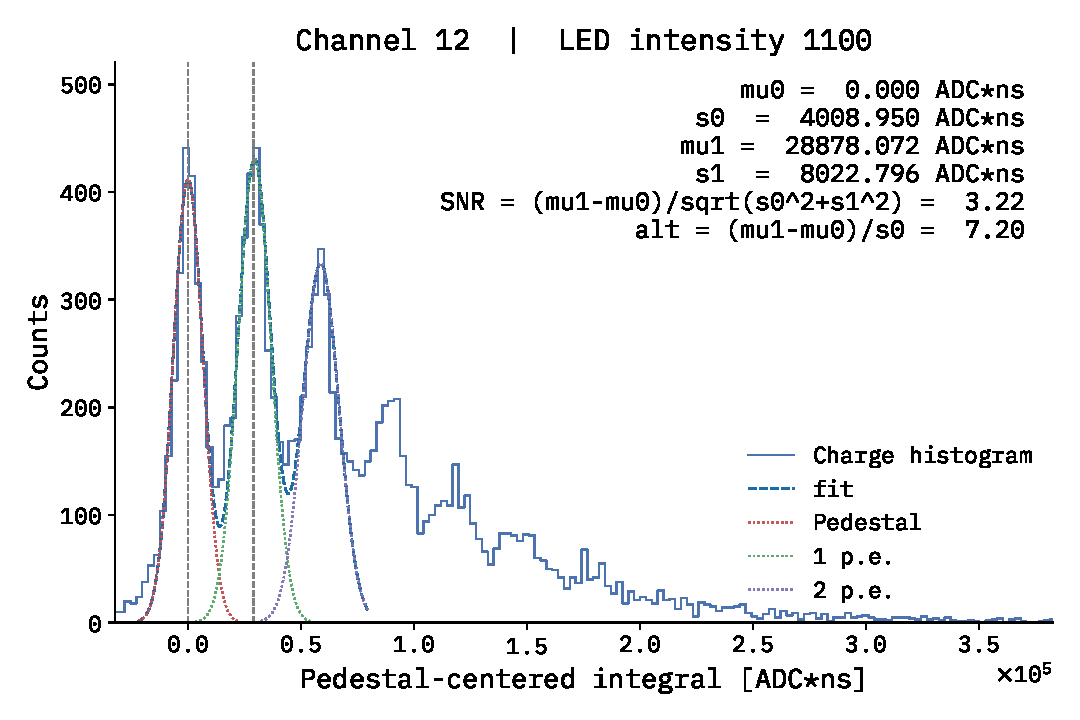
\includegraphics[width=0.23\linewidth]{figures/hd_ch12_1100.pdf}\hfill
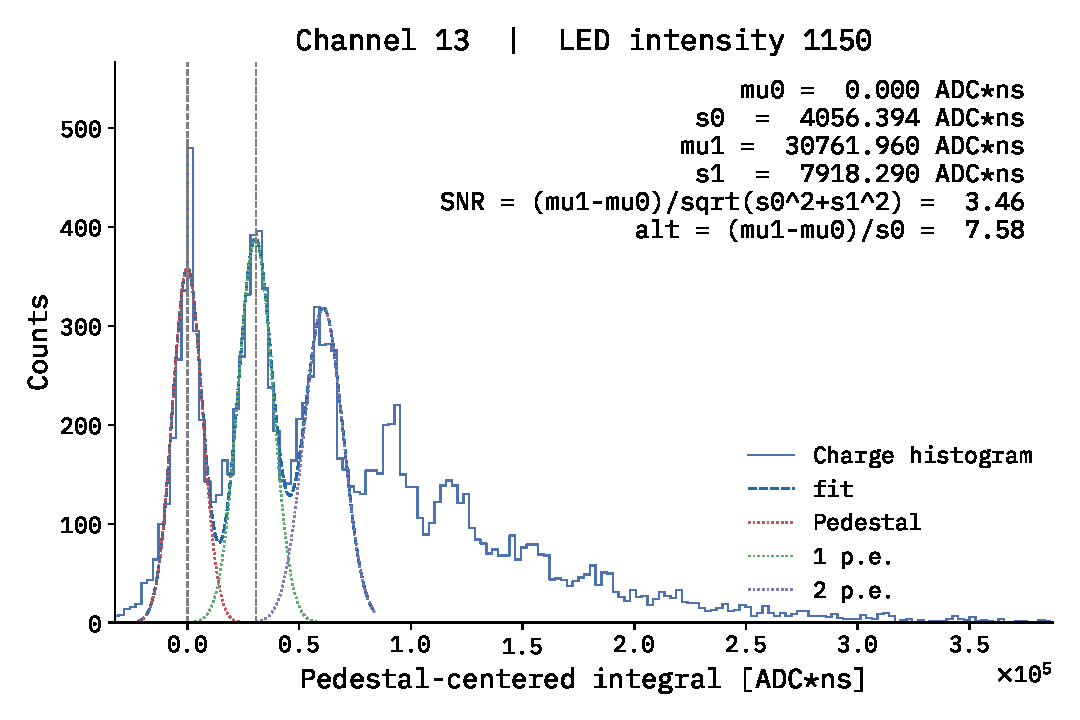
\includegraphics[width=0.23\linewidth]{figures/hd_ch13_1150.pdf}\hfill
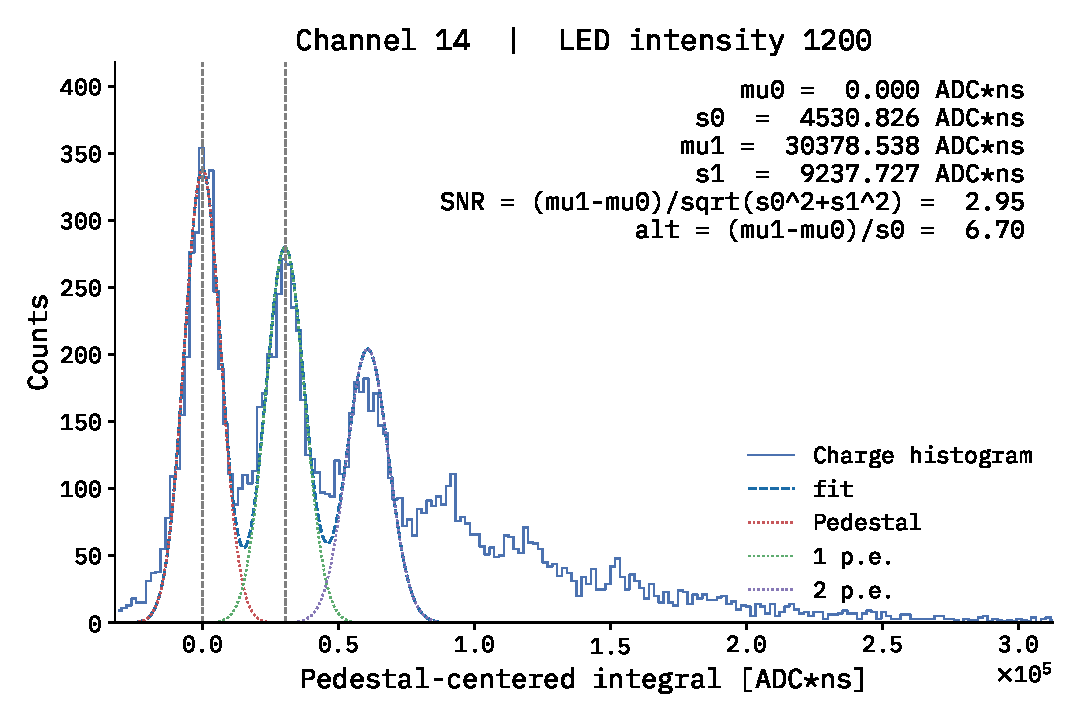
\includegraphics[width=0.23\linewidth]{figures/hd_ch14_1200.pdf}\hfill
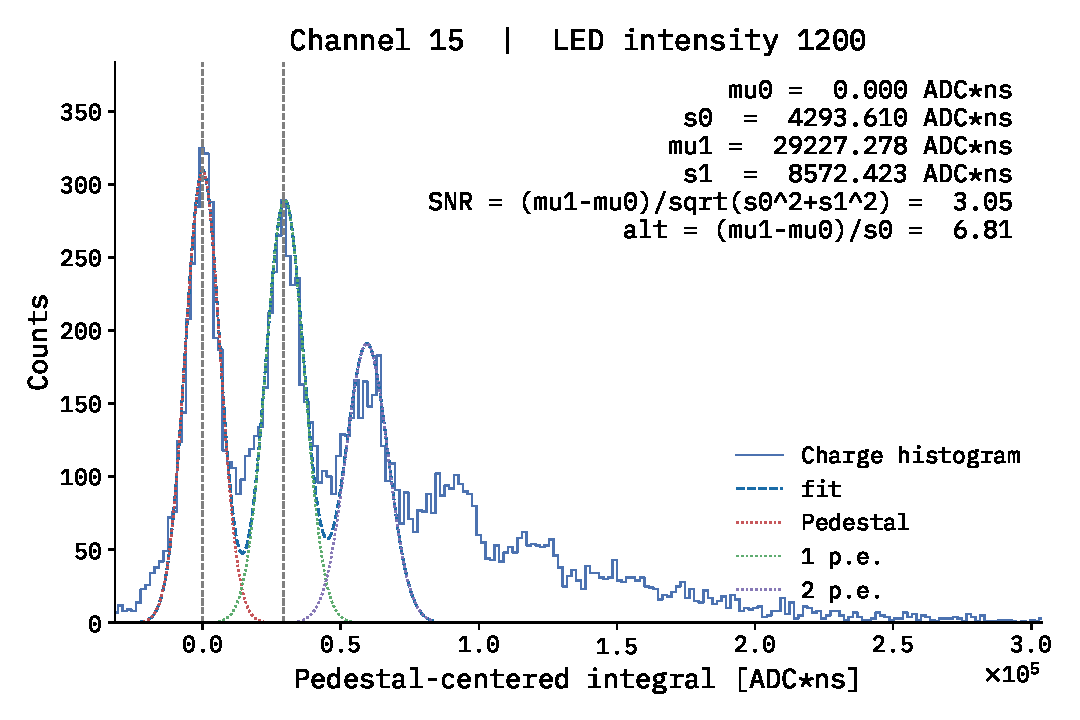
\includegraphics[width=0.23\linewidth]{figures/hd_ch15_1200.pdf}
\end{frame}

\begin{frame}{367 nm scans: dynamic range and saturation}
\small
\begin{itemize}
  \item The 367 nm scans were \textbf{not} used to set the SPE working point.
  \item They were used as the \textbf{high-light dataset} to drive the system toward dynamic-range and saturation studies.
  \item In practice, the 367 nm scans explored wide LED settings at fixed FE configurations, mainly to test when the response leaves the linear / low-occupancy regime.
  \item This complements the 270 nm low-light scans: 270 nm for SPE-oriented operation, 367 nm for high-occupancy / saturation behavior.
\end{itemize}


\vspace{0.5mm}
\scriptsize
Representative HD examples from the March 18 remote 367 nm scan.
\end{frame}

\begin{frame}{Current dataset status}
\footnotesize
\begin{itemize}
  \item \textbf{Noise / no LED:} the dataset is broad and includes multiple electrical configurations, dark VGAIN scans, and oscilloscope captures.
  \item \textbf{VD low-light scans:} channels 0--3 and 4--7 have dedicated 270 nm working-point scans and retakes.
  \item \textbf{HD low-light scans:} channels 12--15 have explicit fingerplot examples and a dedicated 270 nm VGAIN-bias matrix.
  \item \textbf{High-light scans:} 367 nm scans exist and were used for dynamic-range / saturation studies.
  \item \textbf{Remaining systematic gap:} the main channel family still awaiting a comparable dedicated campaign is SoF / AFE2, channels 16--23.
\end{itemize}

\vspace{1mm}
\textbf{Practical interpretation}
\begin{itemize}
  \item We already have a useful dataset for a first CE/WE performance discussion.
  \item The next priority is not more depth on already-covered VD/HD examples, but systematic completion of the SoF channel family.
\end{itemize}
\end{frame}

\end{document}
